\begin{frame}
\frametitle{Binary neutron star mergers as an engine for short GRBs}
\hspace{-0.5cm}
\begin{minipage}[]{0.5\textwidth}
\begin{itemize}
\item Luminosity $L \simeq 10^{48} \mathrm{erg\, s^{-1}}$
\item Burst duration $< 2$s
\item Black hole as a result of the merger surrounded by accretion disk generates a jet
\item r-process nucleosynthesis in the disk and the jet
\item Ideal multi-messenger source in neutrinos, gravitational waves, and X-rays
\end{itemize}
\end{minipage}
%\hspace{0.5cm}
\hspace{0.5cm}
\begin{minipage}[]{0.4\textwidth}
\begin{minipage}[]{\textwidth}
%\hspace{-1.0cm}
%\begin{figure}
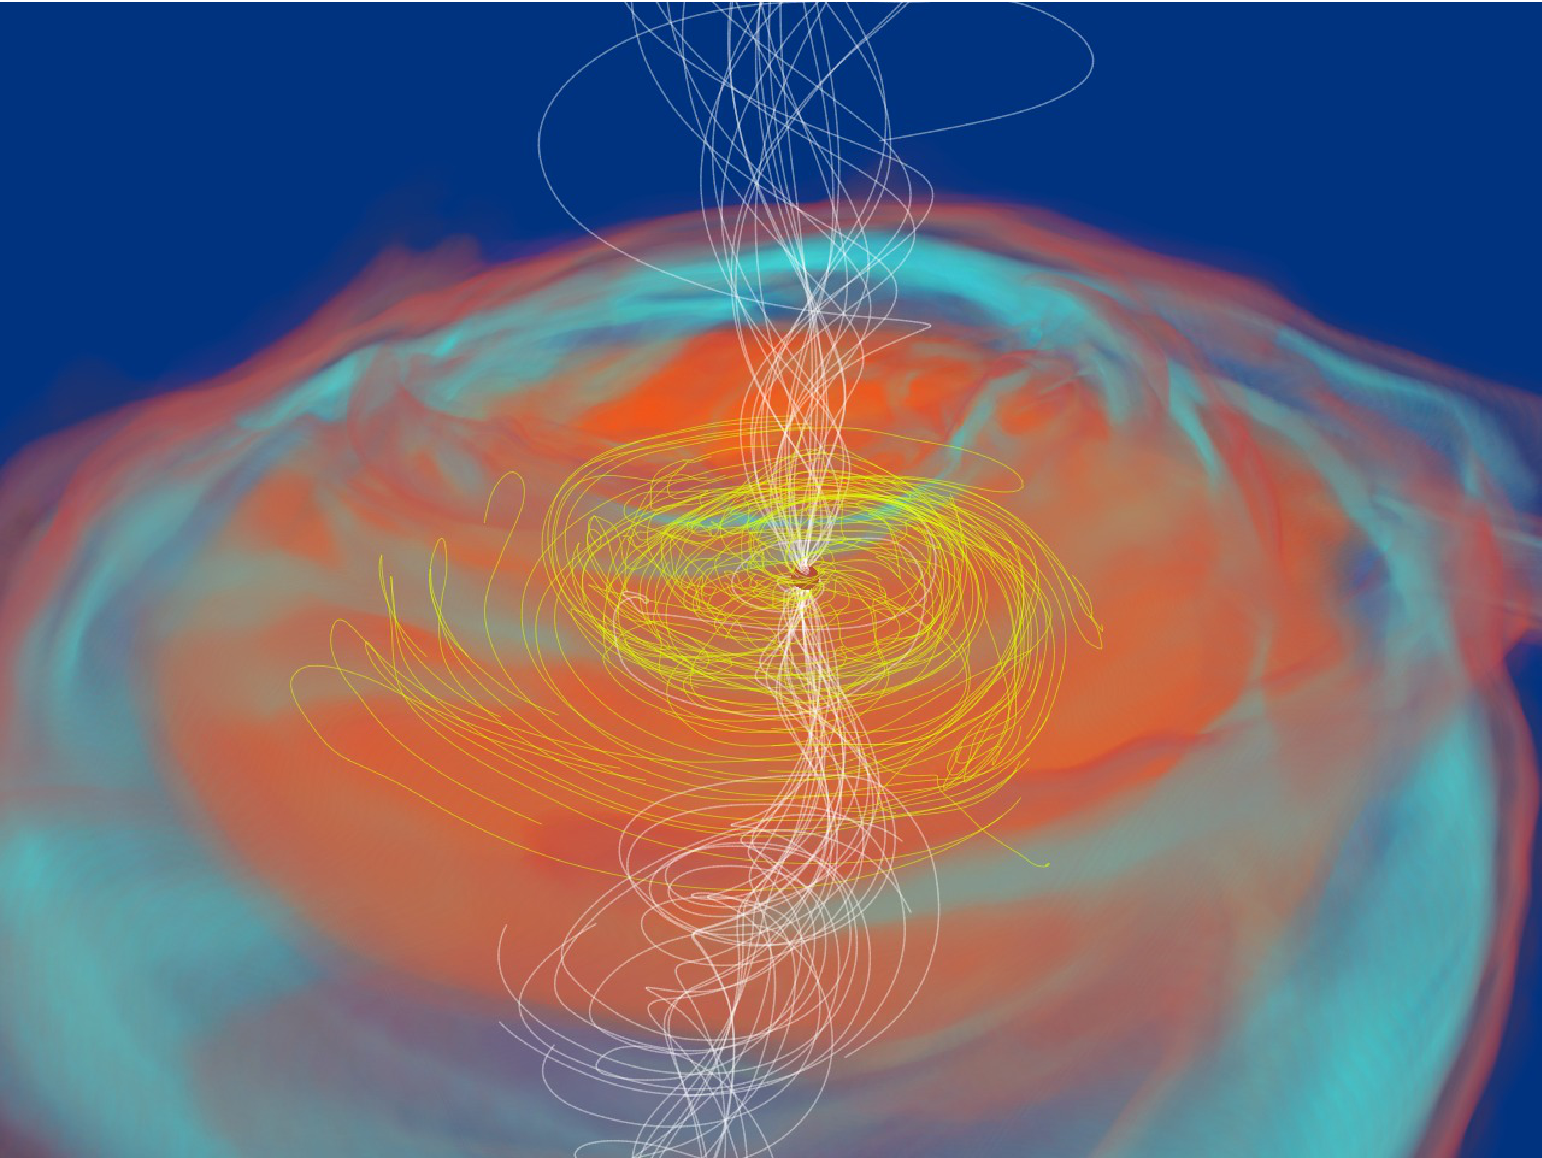
\includegraphics[width=5.0cm]{./etienne.png}
%\end{figure}
\end{minipage}

\begin{minipage}[]{\textwidth}
\small [Etienne et al. 2013]
\end{minipage}
\end{minipage}

\end{frame}



\begin{frame}
\frametitle{Core collapse supernovae}
\hspace{-0.5cm}
\begin{minipage}[]{0.45\textwidth}
\begin{itemize}
\item Death of massive stars; explosion energies up to $10^{53} \mathrm{erg\, s^{-1}}$
\item 99 \% of that energy released in neutrinos
\item Explosive nucleosynthesis enriches the interstellar medium with heavy elements
\item Typical transient astronomy sources, lightcurves powered by radioactive decay of ejected material  
\end{itemize}
\end{minipage}
%\hspace{0.5cm}
\hspace{0.5cm}
\begin{minipage}[]{0.4\textwidth}
\begin{minipage}[]{\textwidth}
%\hspace{-1.0cm}
%\begin{figure}
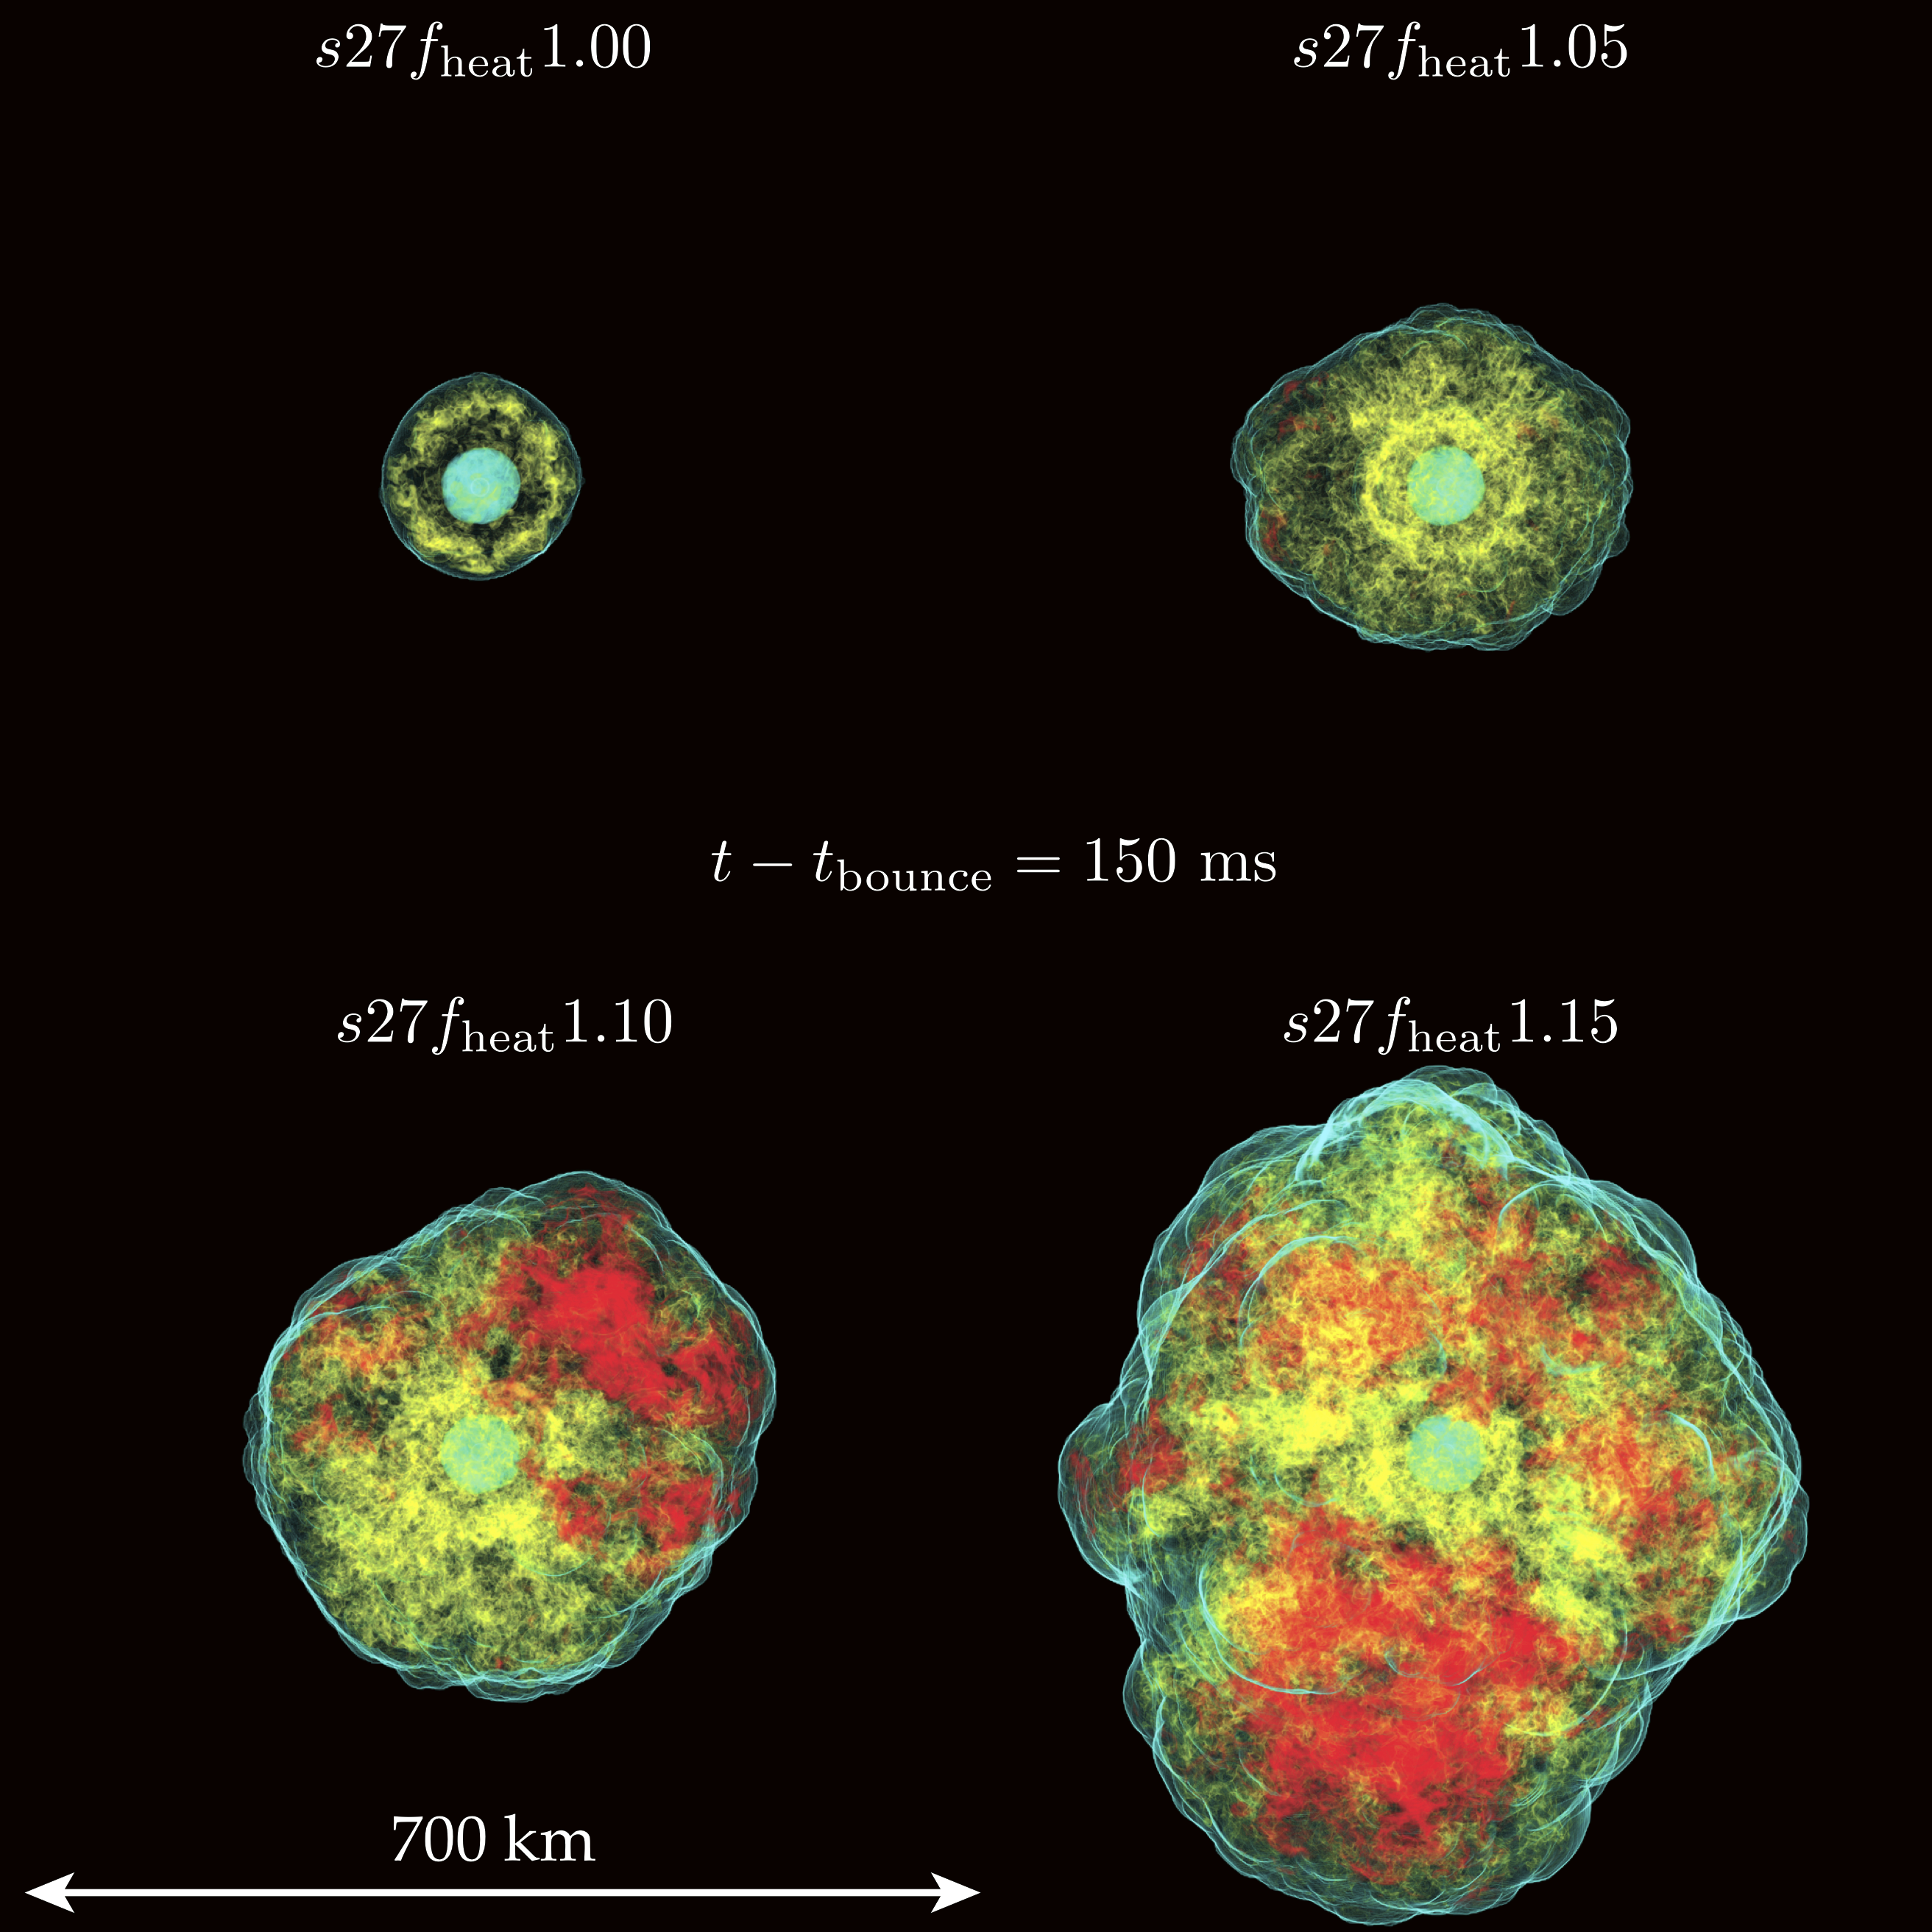
\includegraphics[width=5.0cm]{./s27WHW02_fh_all_vol_drasco.png}
%\end{figure}
\end{minipage}

\begin{minipage}[]{\textwidth}
\small [Ott et al. 2012]
\end{minipage}
\end{minipage}

\end{frame}

\begin{frame}
\frametitle{Supernova + long gamma ray burst connection}
\begin{minipage}[]{0.45\textwidth}
A fraction of type Ic-bl supernovae are observed in combination with a long gamma ray burst/x-ray flash: 
\end{minipage} 
\hspace{0.5cm}
\vspace{0.5cm}
\begin{minipage}[]{0.45\textwidth}
\begin{minipage}[]{\textwidth}
%\begin{figure}
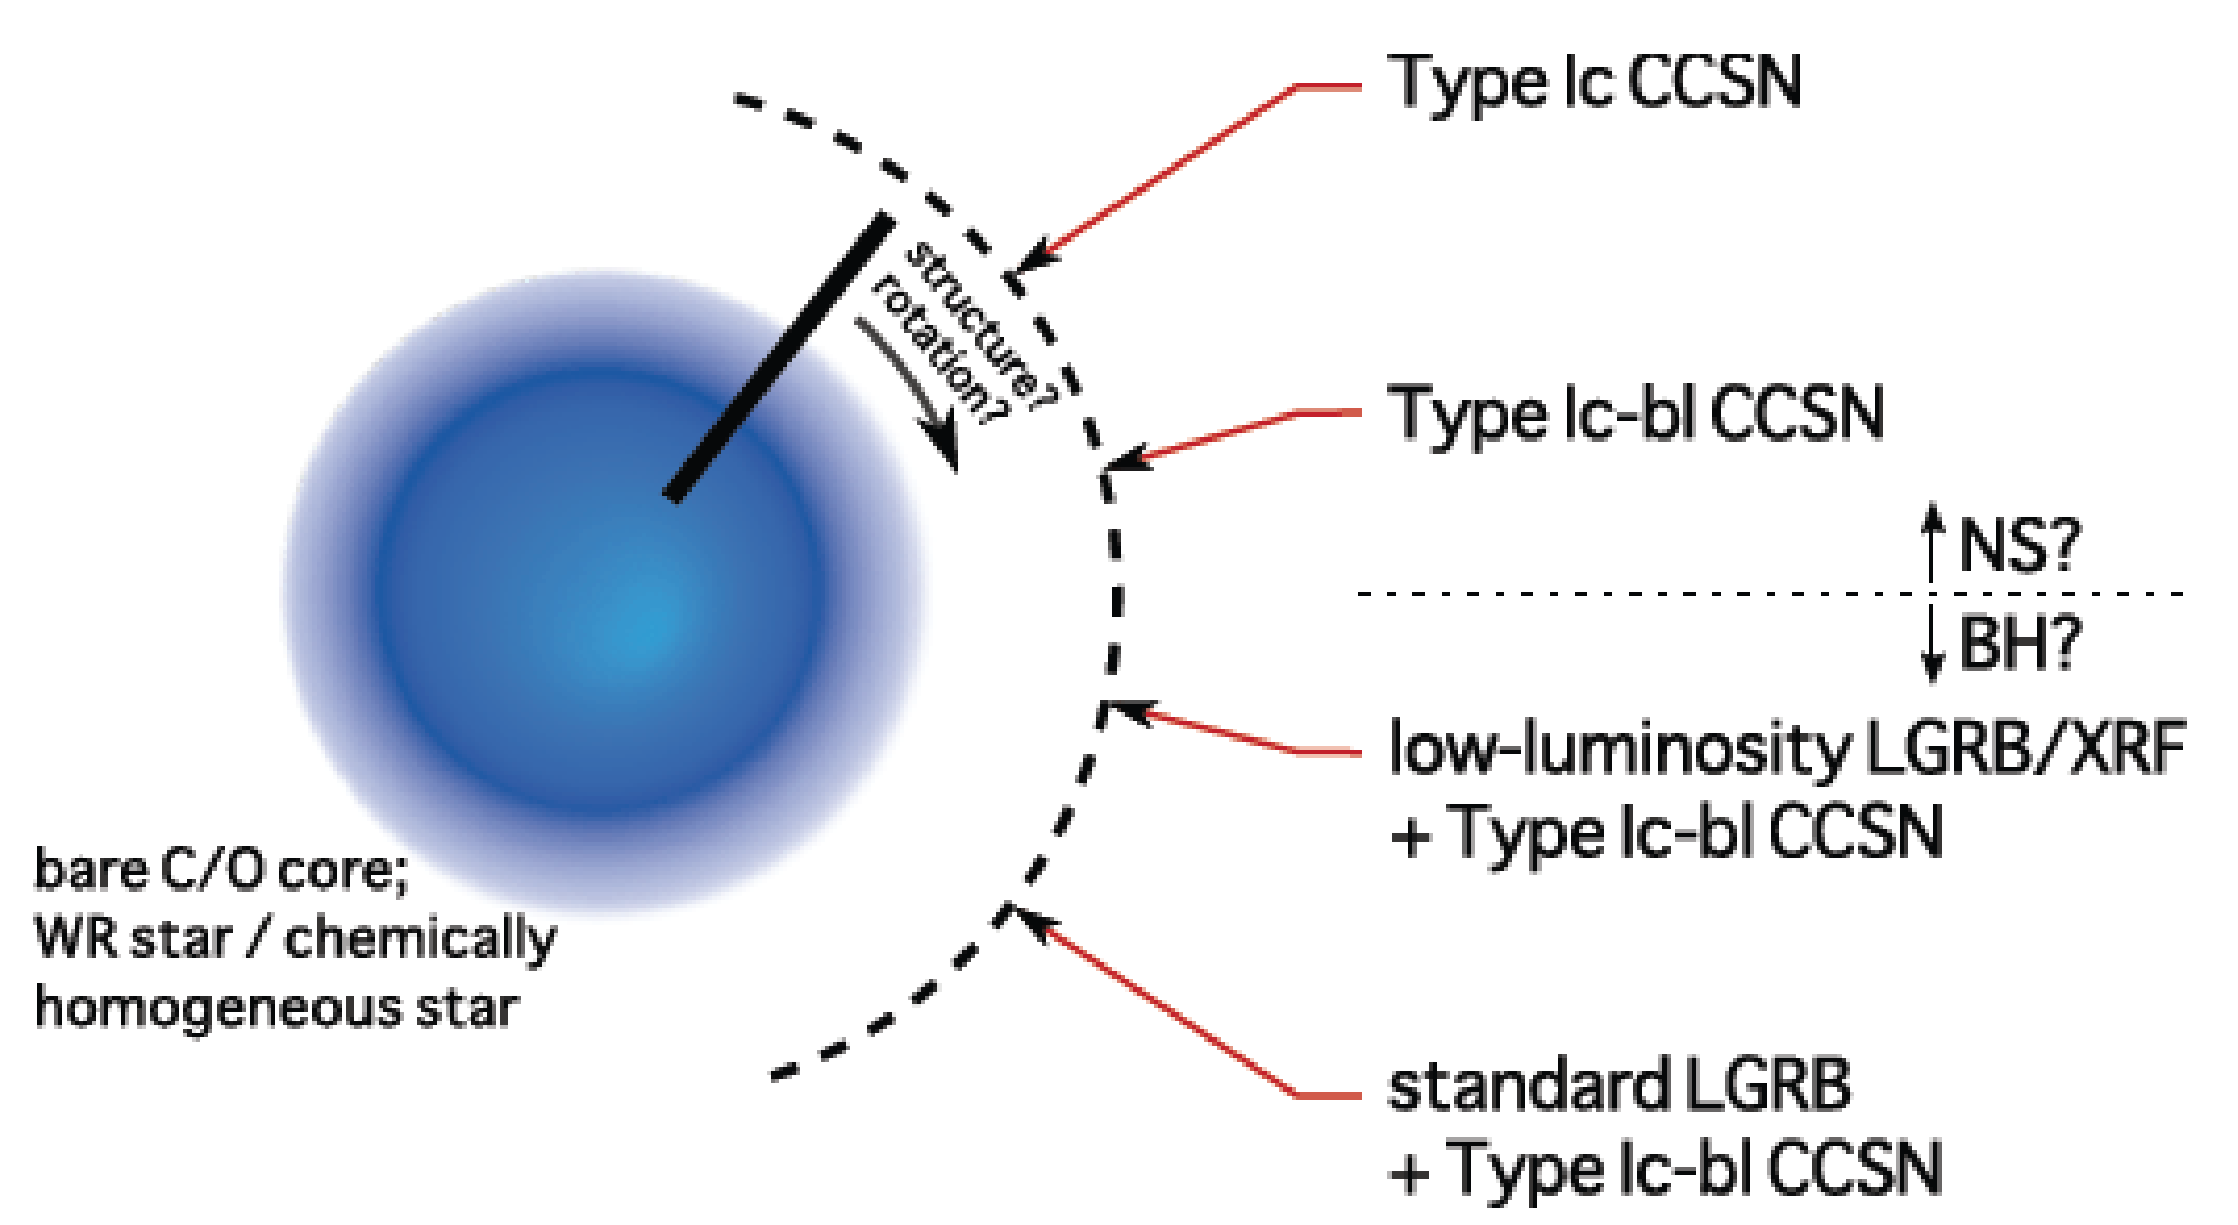
\includegraphics[width=5.0cm]{./dial.png}
%\end{figure}
\end{minipage}
\end{minipage}

\vspace{0.5cm}
\begin{minipage}[]{\textwidth}
What is the engine behind this process and how does it depend on the progenitor parameters? Proto-magnetar or accretion powered collapsar?
\end{minipage}
\end{frame}

\begin{frame}
\frametitle{Stellar collapse / neutron star merger simulations}
\begin{center}
\vspace{-0.5cm}
{\bf Stellar collapse:}
\begin{itemize}
\item Jet propagation speed, instabilities and asymmetries in the jet geometry 
\item Tracer particles to track the explosive nucleosynthesis along the outflows of stellar material
\item Composition and mass of the ejected material and asymmetries in the ejecta
\end{itemize}
\vspace{0.5cm}
{\bf Neutron star mergers:}
\begin{itemize}
\item Modeling of merger, accretion phase, black hole and jet formation
\item r-process nucleosynthesis in ejected material  
\end{itemize}
\end{center}
\end{frame}

\begin{frame}
\frametitle{Modeling:}
\begin{center}
%\vspace{0.5cm}
\begin{itemize}
\item (Ideal) MHD: fluid and magnetic field dynamics 
\item GR: space-time dynamics, neutron star radius
\item Realistic nuclear tabulated EOS: Nuclear interactions
\item Neutrino physics and transport: Neutrino interactions (heating, cooling, etc)
\item Computational infrastructure: Adaptive mesh-refinement (AMR)
\item Multi-D modeling (turbulence, convection, MRI) in massively parallel environments needed!
\end{itemize}
\vspace{0.5cm} 
\bf{We use our open-source code \textit{GRHydro} which is part of the \textit{Einstein Toolkit (www.einsteintoolkit.org)}}!
\end{center}
\end{frame}

\frame { \frametitle{Einstein Toolkit}
  \begin{wrapfigure}{R}{0.15\textwidth}
    \hspace{-20pt}
    \begin{center}
      \includegraphics[width=0.15\textwidth]{et_logo}
    \end{center}
    \vspace{-20pt}
  \end{wrapfigure}
  $ $

\textbf{The Einstein Toolkit} is
\begin{itemize}
  \item an open software scientific tool kit for relativistic astrophysics. 
  \item to provide the core computational tools that can
    \begin{itemize}
       \item enable new science, 
       \item broaden our community, 
       \item facilitate interdisciplinary research,
       \item take advantage of emerging petascale computers and advanced cyberinfrastructure.
    \end{itemize}
  \item available at \url{http://einsteintoolkit.org/}
\end{itemize}
}

